\section{$\lambdaLVar$: syntax and semantics}\label{s:lvars-lambdalvar}

\lk{Figures~\ref{f:lvars-lambdaLVar-syntax} and
  \ref{f:lvars-lambdaLVar-semantics} are an attempt at cutting the
  handlers/quiescence/freezing stuff out of the POPL formalism, but it
  probably needs to be looked at more closely.}

\FigLambdaLVarGrammar

\FigLambdaLVarSemantics

The syntax and operational semantics of $\lambdaLVar$ appear in
Figures~\ref{f:lvars-lambdaLVar-syntax} and
\ref{f:lvars-lambdaLVar-semantics}, respectively.  Both the
syntax and semantics are parameterized by the lattice $D$.  The
reduction relation $\parstepsto$ is defined on \emph{configurations}
$\config{S}{e}$ comprising a store and an expression.  The \emph{error
  configuration}, written $\error$, is a unique element added to the
set of configurations, but $\config{\topS}{e}$ is equal to $\error$
for all expressions $e$.  The metavariable $\conf$ ranges over
configurations.

$\lambdaLVar$ uses a reduction semantics based on \emph{evaluation
  contexts}.  The {\sc E-Eval-Ctxt} rule is a standard context rule,
allowing reductions to apply within a context.  The choice of context
determines where evaluation can occur; in $\lambdaLVar$, the order of
evaluation is nondeterministic (that is, a given expression can
generally reduce in more than one way), and so it is generally
\emph{not} the case that an expression has a unique decomposition into
redex and context.  For example, in an application $\app{e_1}{e_2}$,
either $e_1$ or $e_2$ might reduce first.  The nondeterminism in
choice of evaluation context reflects the nondeterminism of scheduling
between concurrent threads, and in $\lambdaLVar$, the arguments to
@get@, @put@, and application expressions are \emph{implicitly}
evaluated concurrently.

The rules {\sc E-New}, {\sc E-Put}/{\sc E-Put-Err}, and {\sc E-Get}
respectively express the semantics of the @new@, @put@, and @get@
operations described in
Section~\ref{subsection:lvars-communication-primitives}.  The {\sc
  E-New} rule creates a new binding in the store and returns a pointer
to it; the side condition $l \notin \dom{S}$ ensures that $l$ is a
fresh location.  The {\sc E-Put} rule updates the store and returns
$\unit$, the unit value.  The {\sc E-Put-Err} rule applies when a
@put@ to a location would take its state to $\top$; in that case, the
semantics steps to $\error$.  The incompatibility of the threshold set
argument to @get@ is enforced in the {\sc E-Get} rule by the
$\incomp{T}$ premise, which requires that the least upper bound of any
two distinct elements in $T$ must be $\top$.

\subsection{Fork-join parallelism}\label{subsection:fork-join}

$\lambdaLVar$ has a call-by-value semantics: arguments must be fully
evaluated before function application ($\beta$-reduction, modeled by
the {\sc E-Beta} rule) can occur.  I exploit this property to define a
syntactic sugar @let par@ for \emph{parallel composition}, which
computes two subexpressions $e_1$ and $e_2$ in parallel before
computing $e_3$:\TODO{Figure out why the typesetting here is wonky.}
\begin{displaymath}
\begin{minipage}[b]{2in}
  \begin{equation*}
\begin{split}
& \LETPAR ~x = e_1 \\ 
& \letparspace ~y = e_2 \\
& \letspace \IN~e_3 
\end{split}
\end{equation*}
\end{minipage}
\begin{minipage}[b]{1in}
\centering
$\defeq$
\end{minipage}
\begin{minipage}[b]{2in}
\begin{equation*}
  \app{(\app{(\lam{x}{(\lam{y}{e_3})})}{e_1})}{e_2}
\end{equation*}
\end{minipage}
\end{displaymath}

Although $e_1$ and $e_2$ can be evaluated in parallel, $e_3$ cannot be
evaluated until both $e_1$ and $e_2$ are values, because the
call-by-value semantics does not allow $\beta$-reduction until the
operand is fully evaluated, and because it further disallows reduction
under $\lambda$-terms (sometimes called ``full $\beta$-reduction'').
In the terminology of parallel programming, a @let par@ expression
executes both a \emph{fork} and a \emph{join}.  Indeed, it is common
for fork and join to be combined in a single language construct, for
example, in languages with parallel tuple expressions such as
Manticore~\cite{manticore_parallel_tuples}.

\begin{figure}[tb]
  \centering 
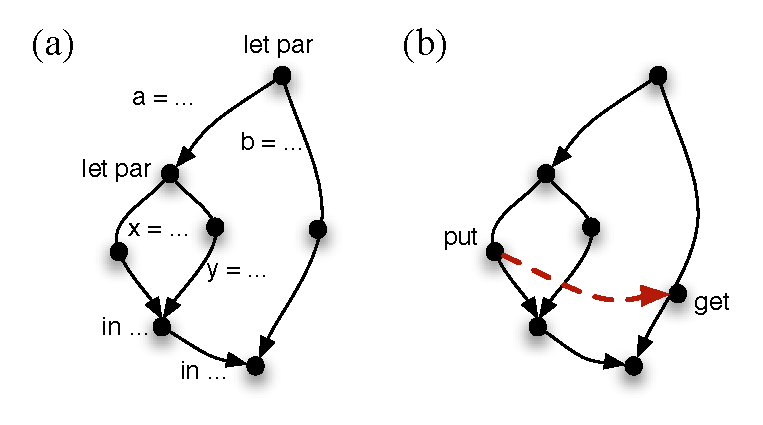
\includegraphics[width=4in]{chapter2/figures/SeriesParallel.pdf} 
\caption{A series-parallel graph induced by parallel
  $\lambda$-calculus evaluation (a); a non-series-parallel graph
  induced by \lstinline|put|/\lstinline|get| operations (b).}
  \label{f:series-parallel}
\end{figure}

Since @let par@ expresses \emph{fork-join} parallelism, the evaluation
of a program comprising nested @let par@ expressions would induce a
runtime dependence graph like that pictured in
Figure~\ref{f:series-parallel}(a).  The $\lambdaLVar$ language (minus
@put@ and @get@) can support any \emph{series-parallel} dependence
graph.  Adding communication through @put@ and @get@ introduces
``lateral'' edges between branches of a parallel computation, as in
Figure~\ref{f:series-parallel}(b).  This adds the ability to construct
arbitrary non-series-parallel dependency graphs, just as with
\emph{first-class futures}~\cite{beyond-nested-workstealing}.

Because the $\lambdaLVar$ semantics does not reduce under
$\lambda$-terms, we can sequentially compose $e_1$ before $e_2$ by
writing $\letexp{\_}{e_1}{e_2}$, which desugars to
$\app{(\lam{\_}{e_2})}{e_1}$.  Sequential composition is useful for,
for instance, allocating a new LVar before beginning a sequence of
side-effecting @put@ and @get@ operations on it.

\subsection{Programming with \lstinline|put| and \lstinline|get|}\label{subsection:lvars-programming-with-put-and-get}

For my first example of a $\lambdaLVar$ program, I will choose the
elements of the lattice to be pairs of natural-number-valued IVars, as
shown in Figure~\ref{f:lattice-examples}(b).  I can then write the
following program:
\begin{equation}
\begin{split}
& \letexp{p}{\NEW}{ \\
& \letspace \letexp{\_}{\putexp{p}{(3,4)}}{ \\
& \letspace \letspace \letexp{v_1}{\getexp{p}{\stateset{(\bot, n) \setsep n \in \mathbb{N}}}}{ \\
& \letspace \letspace \letspace \dots v_1 \dots}}}
\end{split}
\label{e:getSnd}
\end{equation}
This program creates a new LVar $p$ and stores the pair $(3, 4)$ in
it.  $(3,4)$ then becomes the \emph{state} of $p$.  The premises of
the {\sc E-Get} reduction rule hold: $S(p) = (3,4)$; the threshold
set $T = \stateset{(\bot, n) \setsep n \in \mathbb{N}}$ is a pairwise
incompatible subset of $D$; and there exists an element $d_1 \in T$
such that $d_1 \userleq (3,4)$.  In particular, the pair $(\bot, 4)$
is a member of $T$, and $(\bot,4) \userleq (3,4)$.  Therefore,
$\getexp{p}{\stateset{(\bot, n) \setsep n \in \mathbb{N}}}$ returns
the pair $(\bot,4)$.

Since threshold sets can be cumbersome to read, I'll define some
shorthands $\GETFST$ and $\GETSND$ for working with this lattice of
pairs:
\begin{align*}
\getfstexp{p} \defeq \getexp{p}{\stateset{(n, \bot) \setsep n \in
    \mathbb{N}}} \\
\getsndexp{p} \defeq \getexp{p}{\stateset{(\bot, n) \setsep n \in
    \mathbb{N}}}
\end{align*}
The approach I take here for pairs generalizes to arrays of arbitrary
size, with \emph{streams} being the special case of unbounded arrays
where consecutive locations are written.

\subsubsection{Querying incomplete data structures}

It is worth noting that $\getsndexp{p}$ returns a value even if the
first entry of $p$ is not filled in.  For example, if the @put@
expression in the second line of \eqref{e:getSnd} had been
$\putexp{p}{(\bot,4)}$, the @get@ expression would still return
$(\bot,4)$.  It is therefore possible to safely query an incomplete
data structure---say, an object that is in the process of being
initialized by a constructor.  However, I \emph{cannot} define a
$\GETFSTORSND$ function that returns if either entry of a pair is
filled in.  Doing so would amount to passing all of the boxed elements
of the lattice in Figure~\ref{f:lattice-examples}(b) to @get@ as a
single threshold set, which would fail to satisfiy the incompatibility
criterion.

\subsubsection{Blocking reads}

On the other hand, consider the following program:
\begin{equation}
\begin{split}
& \letexp{p}{\NEW}{ \\
& \letspace \letexp{\_}{\putexp{p}{(\bot,4)}}{ \\
& \letspace \letspace \LETPAR ~v_1 = \getfstexp{p} \\
& \letspace \letspace \letparspace \hspace{0.62em}\_~= \putexp{p}{(3,4)} \\
& \letspace \letspace \letspace \IN~ \dots~v_1~\dots }}
\end{split}
\label{e:getSndWithBlock}
\end{equation}
Here $\GETFST$ can attempt to read from the first entry of $p$ before
it has been written to.  However, thanks to @let par@, the $\GETFST$
operation will be evaluated in parallel with a @put@ operation that
will give it a value to read, so $\GETFST$ \emph{blocks} until
$\putexp{p}{(3,4)}$ has been evaluated, at which point the evaluation
of $\getfstexp{p}$ can proceed.

In the operational semantics, this blocking behavior corresponds to
the last premise of the {\sc E-Get} rule not being satisfied.  In
\eqref{e:getSndWithBlock}, although the threshold set $\stateset{(n,
  \bot) \setsep n \in \mathbb{N}}$ is incompatible, the {\sc E-Get}
rule cannot apply because there is no state in the threshold set that
is lower than the state of $p$ in the lattice---that is, we are trying
to @get@ something that is not yet there!  It is only after $p$'s
state is updated that the premise is satisfied and the rule applies.
